% !TeX spellcheck = ru_RU-Russian
% !TeX encoding = UTF-8
\section{Техническое задание}
\subsection{Основание для разработки}

Полное наименование системы: «Программно-информационная система для оценки и контроля знаний».
Основанием для разработки программы является задание на выпускную квалификационную работу.

\subsection{Цель и назначение разработки}

Программно-информационная система предназначена для контроля и оценки знаний обучающихся с целью улучшения процесса обучения.

Задачами данной разработки являются:
\begin{enumerate}
\item Создание модуля для создания новых тестов.
\item Создание модуля для создания вопросов.
\item Создание модуля для редактирования вопросов.
\item Создание модуля для авторизации.
\item Создание модуля для регистрации.
\item Создание модуля для просмотра результатов пройденных тестов.
\item Создание модуля для управления пользователями.
\item Создание модуля для пользователя.
\item Создание модуля для администратора.
\item Реализация системы оценивания по результатам теста.
\item Реализация системы хранения тестов и результатов тестов.
\end{enumerate}

\subsection{Требования к данным программной системы}

Входными данными для системы являются:
\begin{itemize}
    \item данные имеющихся тестов;
    \item данные о зарегистрированных пользователях;
    \item ответы на вопросы теста;
    \item данные администратора.
\end{itemize}

Выходными данными для системы являются:
\begin{itemize}
	\item графическое отображение вопросов тестов;
	\item данные создании/изменении тестов;
	\item данные о новых зарегистрированных/добавленных администратором пользователях;
	\item данные о изменении паролей пользователей;
	\item данные результатов пройденных тестов.
\end{itemize}

\subsection{Функциональные требования к программной системе}

В разрабатываемой программно-информационной системе должно
быть предусмотрено наличие два класса пользователей: пользователь и администратор.

Пользователю должны быть доступны следующие функции программы:
\begin{enumerate}
	\item Авторизация.
	\item Регистрация.
	\item Прохождение выбранного теста.
	\item Просмотр собственных результатов пройденных тестов.
\end{enumerate}

Администратору должны быть доступны следующие функции программы:
\begin{enumerate}
	\item Авторизация.
	\item Изменение пароля администратора.
	\item Прохождение выбранного теста.
	\item Просмотр результатов всех пользователей.
	\item Управление пользователями.
	\item Создание новых тестов.
	\item Редактирование имеющихся тестов.
\end{enumerate}

\subsection{Моделирование вариантов использования}

Для разрабатываемой системы тестирования знаний была реализована модель, которая обеспечивает наглядное представление вариантов использования системы.

Она помогает в физической разработке и детальном анализе взаимосвязей объектов.

Диаграмма вариантов описывает функциональное назначение разрабатываемой системы. То есть это то, что система будет непосредственно делать в процессе своего функционирования. Она является исходным концептуальным представлением системы в процессе ее проектирования и разработки. Проектируемая система представляется в виде ряда прецедентов, предоставляемых системой актерам или сущностям, которые взаимодействуют с системой. Актером или действующим лицом является сущность, взаимодействующая с системой извне (например, человек, техническое устройство). Прецедент служит для описания набора действий, которые система предоставляет актеру.

\clearpage

На рисунке ~\ref{user_precedent_diagram:image} в виде диаграммы прецедентов представлены функциональные требования к системе, доступные для пользователя.

\begin{figure}[H]
	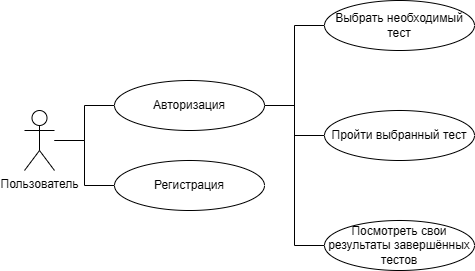
\includegraphics[width=1\linewidth]{диаграмма_прецедентов_пользователь.png}
	\caption{Диаграмма прецедентов пользователя}
	\label{user_precedent_diagram:image}
\end{figure}

\clearpage

На рисунке ~\ref{admin_precedent_diagram:image} представлены дополнительные функциональные требования к системе для администратора.

\begin{figure}[H]
	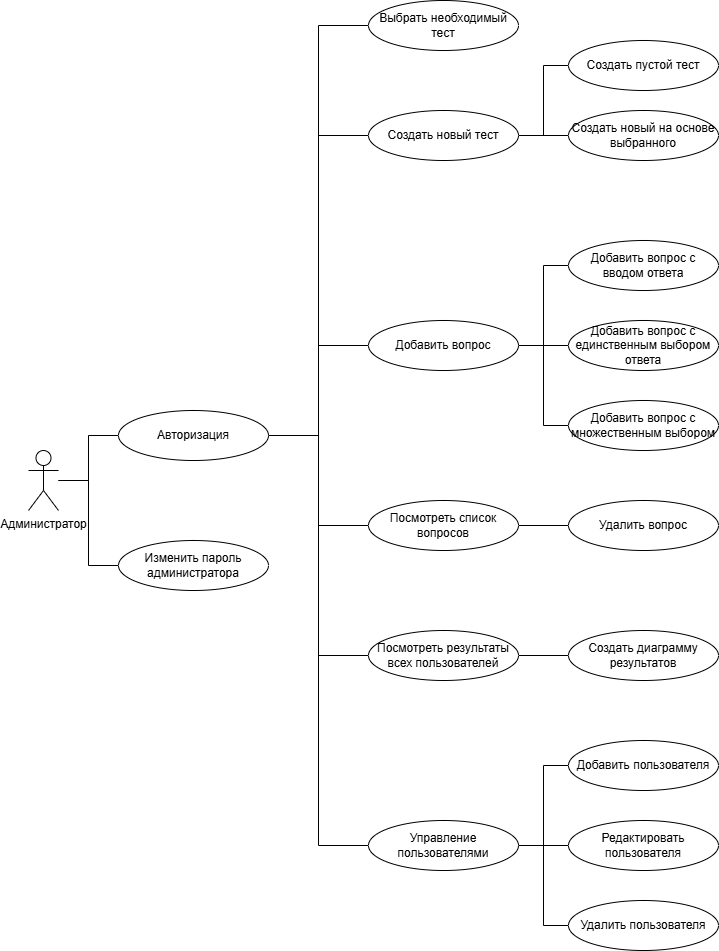
\includegraphics[width=1\linewidth]{диаграмма_прецедентов_администратор.png}
	\caption{Диаграмма прецедентов администратора}
	\label{admin_precedent_diagram:image}
\end{figure}

На основании анализа предметной области в программе должны быть реализованы следующие варианты использования: 
Для пользователя:
\begin{enumerate}
\item ВИ "<Авторизация">. Данный прецедент позволяет пользователю авторизоваться.
\item ВИ "<Регистрация">. Данный прецедент позволяет зарегистрироваться.
\item ВИ "<Выбрать желаемый тест">. Данный прецедент позволяет пользователю выбрать желаемый тест.
\item ВИ "<Пройти выбранный тест">. Данный прецедент позволяет пользователю приступить к прохождению выбранного теста.
\item ВИ "<Добавить вопрос">. Данный прецедент позволяет пользователю добавить вопрос в выбранном тесте.
\item ВИ "<Удалить вопрос">. Данный прецедент позволяет пользователю удалить вопрос в выбранном тесте.
\item ВИ "<Просмотреть результаты">. Данный прецедент позволяет пользователю посмотреть собственные результаты пройденных тестов.
\item ВИ "<Создать новый тест">. Данный прецедент позволяет пользователю создать новый тест.
\end{enumerate}

Для администратора:
\begin{enumerate}
	\item ВИ "<Авторизоваться как администратор">. Данный прецедент позволяет авторизоваться как администратор и получить соответствующие права.
	\item ВИ "<Изменить пароль администратор">. Данный прецедент позволяет изменить пароль администратор. Требуется ввести старый пароль и два раза повторить новый.
	\item ВИ "<Выбрать желаемый тест">. Данный прецедент позволяет администратору выбрать желаемый тест.
	\item ВИ "<Пройти выбранный тест">. Данный прецедент позволяет администратору приступить к прохождению выбранного теста.
	\item ВИ "<Добавить вопрос">. Данный прецедент позволяет администратору добавить вопрос в выбранном тесте. Возможно добавить три варианта вопроса: с вводом ответа, с единственным выбором из имеющихся ответов, с множественным выбором из имеющихся ответов.
	\item ВИ "<Просмотреть набор выбранного теста">. Данный прецедент позволяет администратору посмотреть состав теста.
	\item ВИ "<Удалить вопрос">. Данный прецедент позволяет администратору удалить выбранный вопрос.
	\item ВИ "<Просмотреть результаты">. Данный прецедент позволяет администратору посмотреть результаты пройденных тестов всех пользователей.
	\item ВИ "<Создать новый тест">. Данный прецедент позволяет администратору создать новый тест. Можно создать пустой тест или копировать текущий набор выбранного теста.
	\item ВИ "<Управление пользователями">. Данный прецедент позволяет администратору добавить нового пользователя, удалить или редактировать уже существующего.
\end{enumerate}

\subsubsection{Описание вариантов использования}

Данные варианта использования <<Пройти выбранный тест>>.

Входными данными является выбранный тест, имя пользователя.

Выходными данными прецедента <<Пройти выбранный тест>> являются вопросы с ответами и результат прохождения теста.

Основной исполнитель: Пользователь.

Заинтересованные лица и их требования: Пользователь хочет пройти тест.

Предусловие: поля для ввода имени, ответа на вопрос должны быть заполнены.

Постусловие: приложение проверит введены ли данные, если нет, сообщит об этом пользователю.

Основной успешный сценарий:
\begin{enumerate}
	\item Пользователь запускает программу.
	\item Пользователь проходит авторизацию, введя своё имя.
	\item Пользователь попадает в меню.
	\item Пользователь выбирает желаемый тест.
	\item Пользователь нажимает кнопку <<Пройти тест>>.
	\item Пользователь попадает в окно теста.
	\item Пользователь выбирает или вводит ответы.
	\item Пользователь по окончании теста видит его результат.
	\item Пользователь закрывает приложение.
\end{enumerate}

Данные варианта использования <<Создать новый тест>>.

Входными данными является пароль администратора, данные для нового теста.

Выходными данными прецедента <<Создать новый тест>> являются новый тест с вопросами и ответами.

Основной исполнитель: Администратор.

Заинтересованные лица и их требования: Администратор хочет создать тест и добавить в него вопрос

Предусловие: поля для ввода пароля администратора, текста вопроса и его ответа должны быть заполнены.

Постусловие: приложение проверит введены ли данные, если нет, сообщит об этом администратору.

Основной успешный сценарий:
\begin{enumerate}
	\item Администратор запускает программу.
	\item Администратор проходит авторизацию, введя пароль.
	\item Администратор попадает в меню.
	\item Администратор нажимает кнопку <<Создать тест>>.
	\item Администратор попадает в окно создания теста.
	\item Администратор нажимает кнопку <<Создать новый тест>>.
	\item Администратор нажимает кнопку <<Вернуться в меню>>.
	\item Администратор попадает в меню.
	\item Администратор нажимает кнопку <<Добавить вопрос>>.
	\item Администратор попадает в меню добавления вопроса.
	\item Администратор нажимает кнопку добавить базовый вопрос.
	\item Администратор в окне создания базового вопроса вводит текст и ответ вопроса.
	\item Администратор нажимает кнопку добавить вопрос.
	\item Администратор закрывает приложение.
\end{enumerate}

\paragraph{Вариант использования <<Регистрация>>}

Заинтересованные лица и их требования: пользователь желает зарегистрироваться в приложении.
\newline Предусловие: открыто окно "<Авторизация пользователя">.
\newline Постусловие: создаётся аккаунт нового пользователя на основании введённых данных для регистрации, имени и пароля.
\newline Основной успешный сценарий:
\begin{enumerate}
	\item Пользователь переходит в окно "<Регистрация">.
	\item Приложение отображает соответствующее окно регистрации с полями для ввода имени и пароля (см. рисунок ~\ref{reg_window:image}).
	\item Пользователь заполняет текстовые поля "<Имя"> и "<Пароль"> (см. рисунок ~\ref{reg_data:image}). Данные поля обязательны для заполнения. Имя должно состоять только из символов без цифр, минимум два символа. Имя должно быть уникальным.
	\item Пользователь нажимает кнопку "<Зарегистрироваться">.
	\item Приложение проверяет введённые пользователем имя и пароль. Если данные некорректны, сообщает об этом пользователю. При корректных данных приложение создаёт новый аккаунт и сообщает пользователю об успешной регистрации (см. рисунок ~\ref{successful_reg:image}).
\end{enumerate}

\newpage
\begin{figure}[ht]
	\centering
	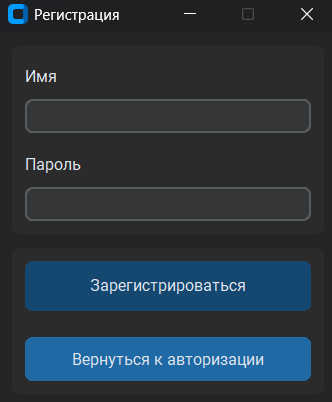
\includegraphics[width=0.5\linewidth]{регистрация.png}
	\caption{Окно "<Регистрация">}
	\label{reg_window:image}
\end{figure}
\begin{figure}[ht]
	\centering
	\includegraphics[width=0.5\linewidth]{регистрация_данные.png}
	\caption{Ввод имени и пароля в окне "<Регистрация">}
	\label{reg_data:image}
\end{figure}
\begin{figure}[ht]
	\centering
	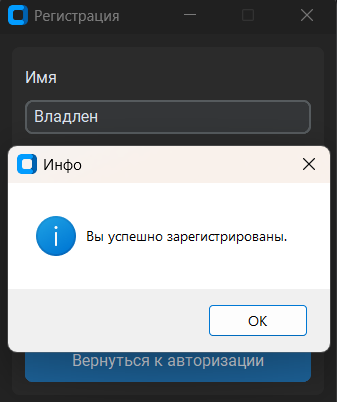
\includegraphics[width=0.5\linewidth]{успешная_регистрация.png}
	\caption{Уведомление об успешной регистрации}
	\label{successful_reg:image}
\end{figure}

\paragraph{Вариант использования <<Авторизация пользователя>>}

Заинтересованные лица и их требования: пользователь желает авторизоваться в приложении.
\newline Предусловие: открыто окно "<Авторизация пользователя">.
\newline Постусловие: авторизация произведена, отображается окно "<Меню пользователя">.
\newline Основной успешный сценарий:
\begin{enumerate}
	\item Пользователь переходит в окно "<Авторизация пользователя"> (см. рисунок ~\ref{user_auth_window:image}).
	\item Приложение отображает соответствующее окно авторизации с полями для ввода имени и пароля.
	\item Пользователь заполняет текстовые поля "<Имя"> и "<Пароль"> (см. рисунок ~\ref{user_auth_data:image}). Данные поля обязательны для заполнения.
	\item Пользователь нажимает кнопку "<Перейти в меню">.
	\item Приложение проверяет введённые пользователем имя и пароль. Если данные некорректны, сообщает об этом пользователю. При корректных данных приложение закрывает текущее окно авторизации и открывает окно "<Меню пользователя"> (см. рисунок ~\ref{user_menu_1:image}).
\end{enumerate}

\begin{figure}[H]
	\centering
	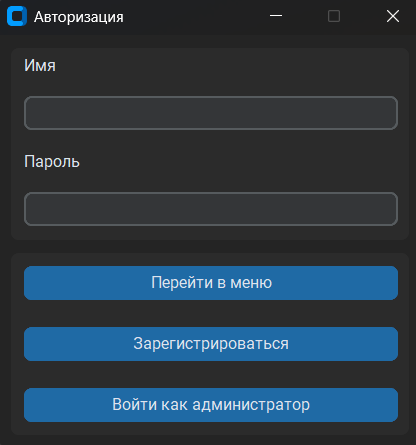
\includegraphics[width=0.6\linewidth]{окно_авторизации_пользователя.png}
	\caption{Окно "<Авторизация пользователя">}
	\label{user_auth_window:image}
\end{figure}
\begin{figure}[H]
	\centering
	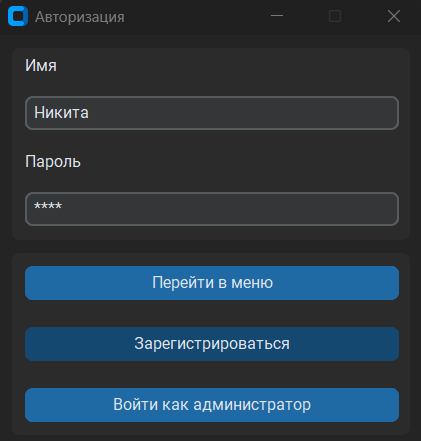
\includegraphics[width=0.6\linewidth]{авторизация_пользователя_данные.png}
	\caption{Ввод имени и пароля пользователя}
	\label{user_auth_data:image}
\end{figure}
\begin{figure}[H]
	\centering
	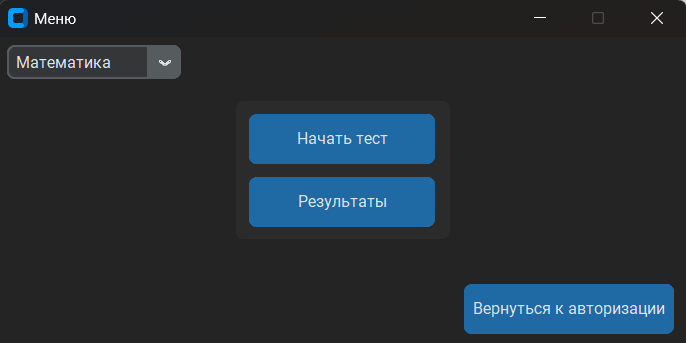
\includegraphics[width=1\linewidth]{меню_п_1.png}
	\caption{Окно "<Меню пользователя">}
	\label{user_menu_1:image}
\end{figure}

\paragraph{Вариант использования <<Тестирование>>}

Заинтересованные лица и их требования: пользователь желает пройти тестирование.
\newline Предусловие: открыто окно "<Меню пользователя"> или "<Меню администратора">.
\newline Постусловие: Даны ответы на все вопросы, приложение отображает результаты тестирования пользователю и сохраняет отчёт результатов.
\newline Основной успешный сценарий:
\begin{enumerate}
	\item Пользователь выбирает желаемый тест в меню с помощью выпадающего списка и нажимает кнопку "<Начать тест"> (см. рисунок ~\ref{user_menu_window:image}).
	\item Приложение отображает окно теста и выводит текст первого вопроса (см. рисунок ~\ref{test_window:image}). Отображение вопроса зависит от его типа: для вопроса с вводом ответа будет создано поле для ввода; для вопроса с единственным выбором ответа будут созданы кнопки с ответам, только одну можно выбрать для ответа; для вопроса с множественным выбором будут созданы кнопки с ответами, можно выбрать сразу несколько ответов.
	\item Пользователь отвечает на вопрос и нажимает кнопку "<Ответить">.
	\item Приложение проверяет ответ пользователя и выводит следующий вопрос. 
	\item Когда пользователь отвечает на последний вопрос, приложение выводит результат прохождения теста и сохраняет его.
\end{enumerate}

\newpage
\begin{figure}[ht]
	\centering
	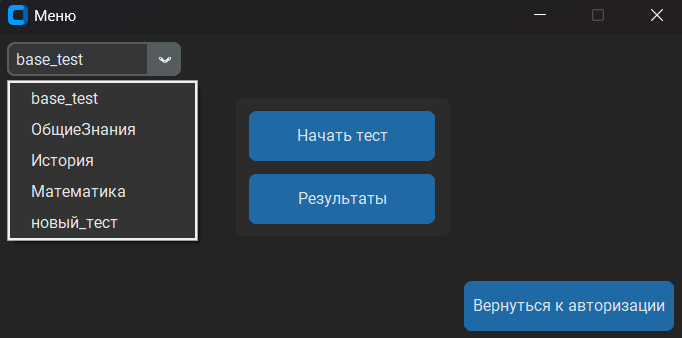
\includegraphics[width=1\linewidth]{меню_пользователя.png}
	\caption{Выбор теста в окне "<Меню пользователя">}
	\label{user_menu_window:image}
\end{figure}
\begin{figure}[ht]
	\centering
	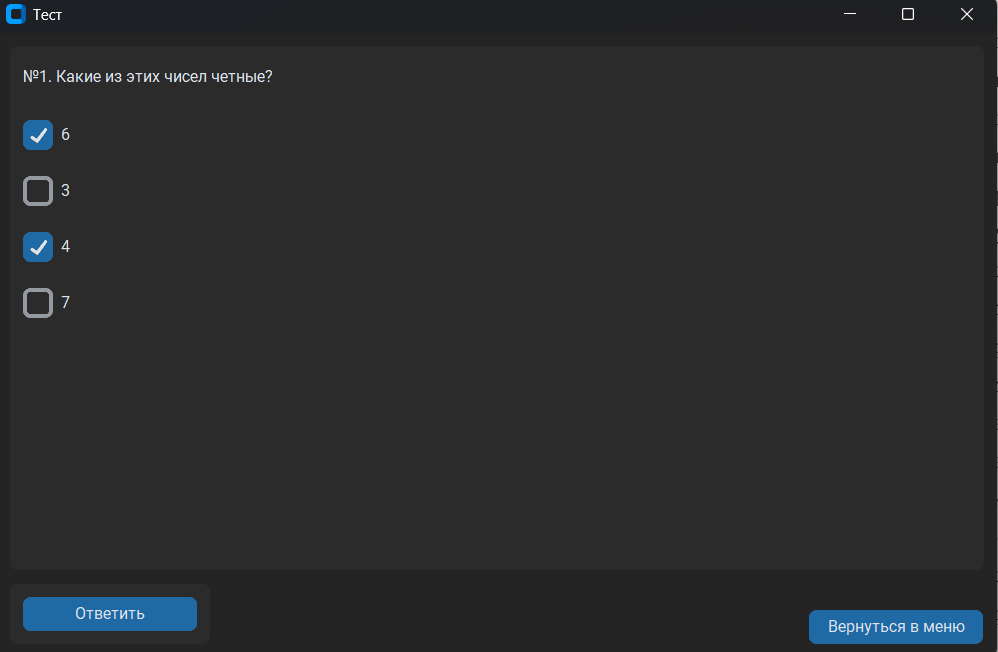
\includegraphics[width=1\linewidth]{тест_1.png}
	\caption{Окно "<Тест">}
	\label{test_window:image}
\end{figure}

\paragraph{Вариант использования <<Просмотр результатов - Пользователь>>}

Заинтересованные лица и их требования: пользователь желает посмотреть все результаты своих пройденных тестов.
\newline Предусловие: открыто окно "<Меню пользователя">.
\newline Постусловие: открыто окно "Результаты", отображены все результаты пройденных тестов пользователя.
\newline Основной успешный сценарий:
\begin{enumerate}
	\item Пользователь переходит в окно "<Результаты">.
	\item Приложение отображает соответствующее окно, где в табличном виде отображает информацию о завершённых тестах пользователя (см. рисунок ~\ref{user_results:image}).
\end{enumerate}

\begin{figure}[H]
	\centering
	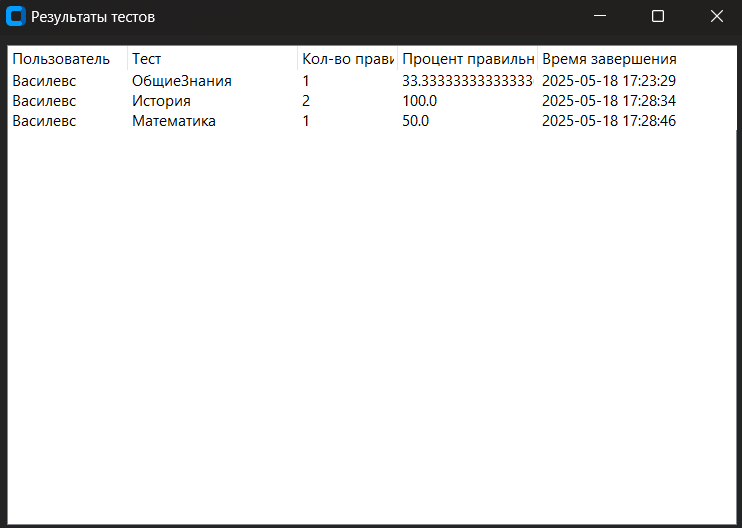
\includegraphics[width=1\linewidth]{результаты_пользователь.png}
	\caption{Окно "<Результаты">}
	\label{user_results:image}
\end{figure}


\paragraph{Вариант использования <<Авторизация администратора>>}

Заинтересованные лица и их требования: администратор желает создать новый тест и добавить в него вопрос.
\newline Предусловие: открыто окно "<Авторизация пользователя">.
\newline Постусловие: Авторизация администратора успешно выполнена. Открыт доступ к "<Меню администратора">.
\newline Основной успешный сценарий:
\begin{enumerate}
	\item Администратор переходит в окно "<Авторизация администратора">.
	\item Приложение отображает окно с двумя кнопками: "<Создать новый тест"> и "<Копировать текущий"> (см. рисунок ~\ref{admin_auth_window:image}).
	\item Администратор вводит пароль и нажимает кнопку "<Перейти в меню"> (см. рисунок ~\ref{admin_password:image}).
	\item Приложение проверяет введённый пароль, сообщает администратору об ошибке, если пароль неверный. Если пароль верный, открывает окно "<Меню администратора"> (см. рисунок ~\ref{admin_menu_1:image}).
\end{enumerate}

\begin{figure}[ht]
	\centering
	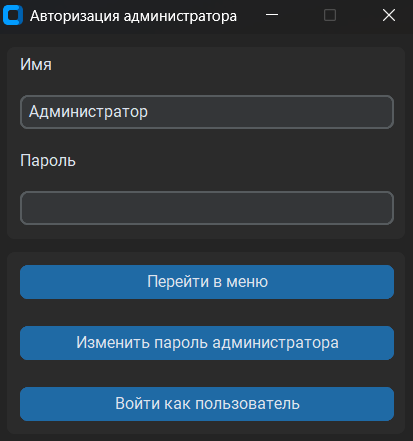
\includegraphics[width=0.5\linewidth]{авторизация_администратора.png}
	\caption{Окно "<Авторизация администратора">}
	\label{admin_auth_window:image}
\end{figure}
\begin{figure}[H]
	\centering
	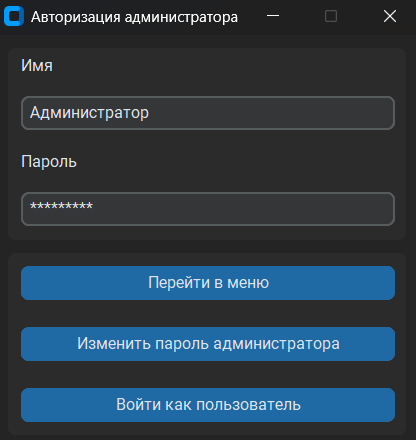
\includegraphics[width=0.5\linewidth]{ввод_пароля_админ.png}
	\caption{Администратор вводит пароль}
	\label{admin_password:image}
\end{figure}
\begin{figure}[H]
	\centering
	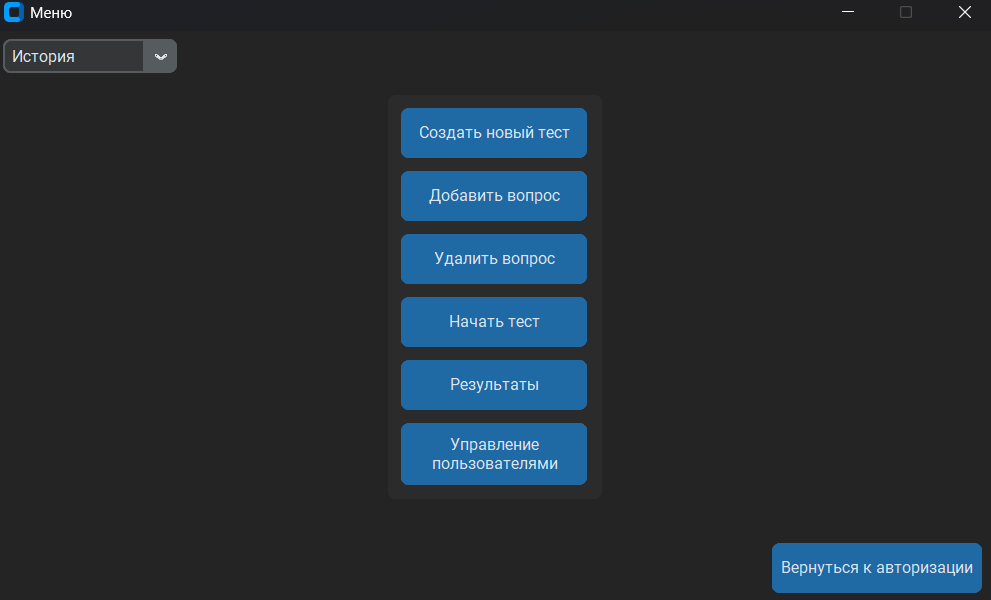
\includegraphics[width=1\linewidth]{меню_администратора.png}
	\caption{Окно "<Меню администратора">}
	\label{admin_menu_1:image}
\end{figure}

\paragraph{Вариант использования <<Изменение пароля администратора>>}

Заинтересованные лица и их требования: администратор желает свой изменить пароль.
\newline Предусловие: открыто окно "<Авторизация администратора">.
\newline Постусловие: Установлен новый пароль для авторизации администратора.
\newline Основной успешный сценарий:
\begin{enumerate}
	\item Администратор переходит в окно "<Изменение пароля">.
	\item Приложение отображает окно с тремя полями для ввода: старый пароль, новый пароль и повторение нового пароля. (см. рисунок ~\ref{admin_password_ch:image}).
	\item Администратор вводит старый пароль, два раза новый и нажимает кнопку "<Изменить пароль"> (см. рисунок ~\ref{admin_password_input:image}).
	\item Приложение проверяет старый пароль, новый пароль и его повтор, сообщает администратору об ошибке, если старый пароль неверный, или новый повторён неправильно, или новый пароль слишком простой. Если данные корректны, изменяет пароль и уведомляет администратора об успешном изменении пароля (см. рисунок ~\ref{admin_password_notif:image}).
\end{enumerate}

\begin{figure}[H]
	\centering
	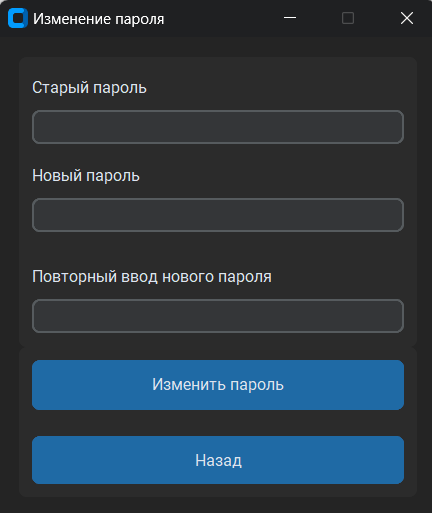
\includegraphics[width=0.6\linewidth]{изм_пароля_администратора.png}
	\caption{Окно "<Изменение пароля">}
	\label{admin_password_ch:image}
\end{figure}
\begin{figure}[H]
	\centering
	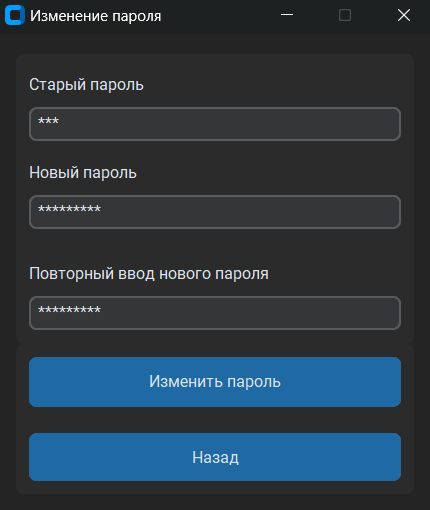
\includegraphics[width=0.6\linewidth]{изм_пар_адм_ввод.png}
	\caption{Ввод старого и нового паролей}
	\label{admin_password_input:image}
\end{figure}
\begin{figure}[H]
	\centering
	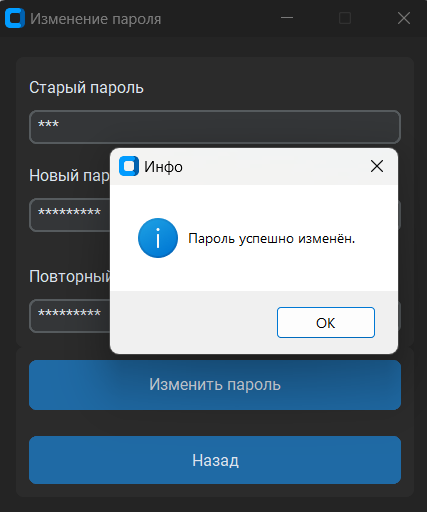
\includegraphics[width=0.6\linewidth]{изм_пар_адм_уведомление.png}
	\caption{Уведомление об успешном изменении пароля}
	\label{admin_password_notif:image}
\end{figure}

\paragraph{Вариант использования <<Просмотр результатов - Администратор>>}

Заинтересованные лица и их требования: администратор желает посмотреть результаты всех пользователей, сформировать диаграмму лучших результатов и сохранить её.
\newline Предусловие: открыто окно "<Меню администратора">.
\newline Постусловие: открыто окно "Результаты", отображены результаты всех пользователей, сформирована диаграмма лучших результатов и сохранена.
\newline Основной успешный сценарий:
\begin{enumerate}
	\item Администратор переходит в окно "<Результаты">.
	\item Приложение отображает соответствующее окно, где в табличном виде отображает информацию о завершённых тестах всех пользователей (см. рисунок ~\ref{admin_results:image}).
	\item Администратор нажимает кнопку "<Диаграмма">, чтобы наглядно увидеть лучшие результаты.
	\item Приложение отображает диаграмму лучших результатов (см. рисунок ~\ref{results_chart:image}).
	\item Администратор нажимает кнопку сохранения диаграммы и в файловом диалоге выбирает место для сохранения (см. рисунок ~\ref{saving_chart:image}).
\end{enumerate}

\begin{figure}[H]
	\centering
	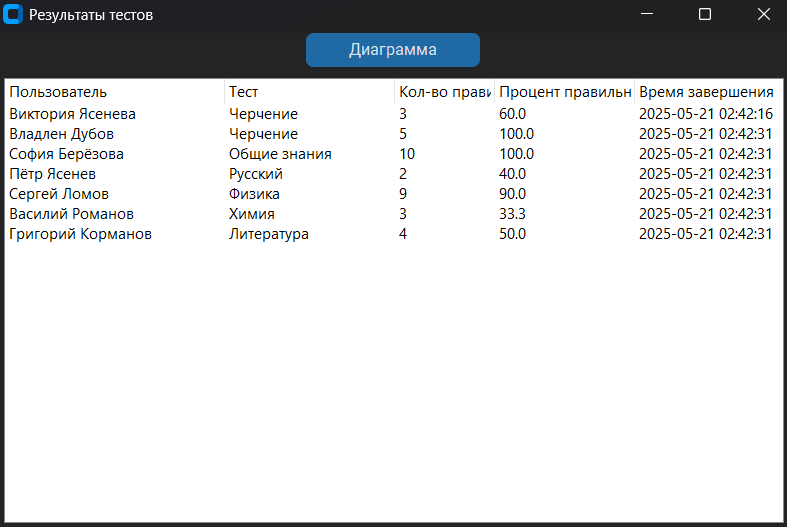
\includegraphics[width=1\linewidth]{результаты_админ.png}
	\caption{Окно "<Результаты">}
	\label{admin_results:image}
\end{figure}
\begin{figure}[H]
	\centering
	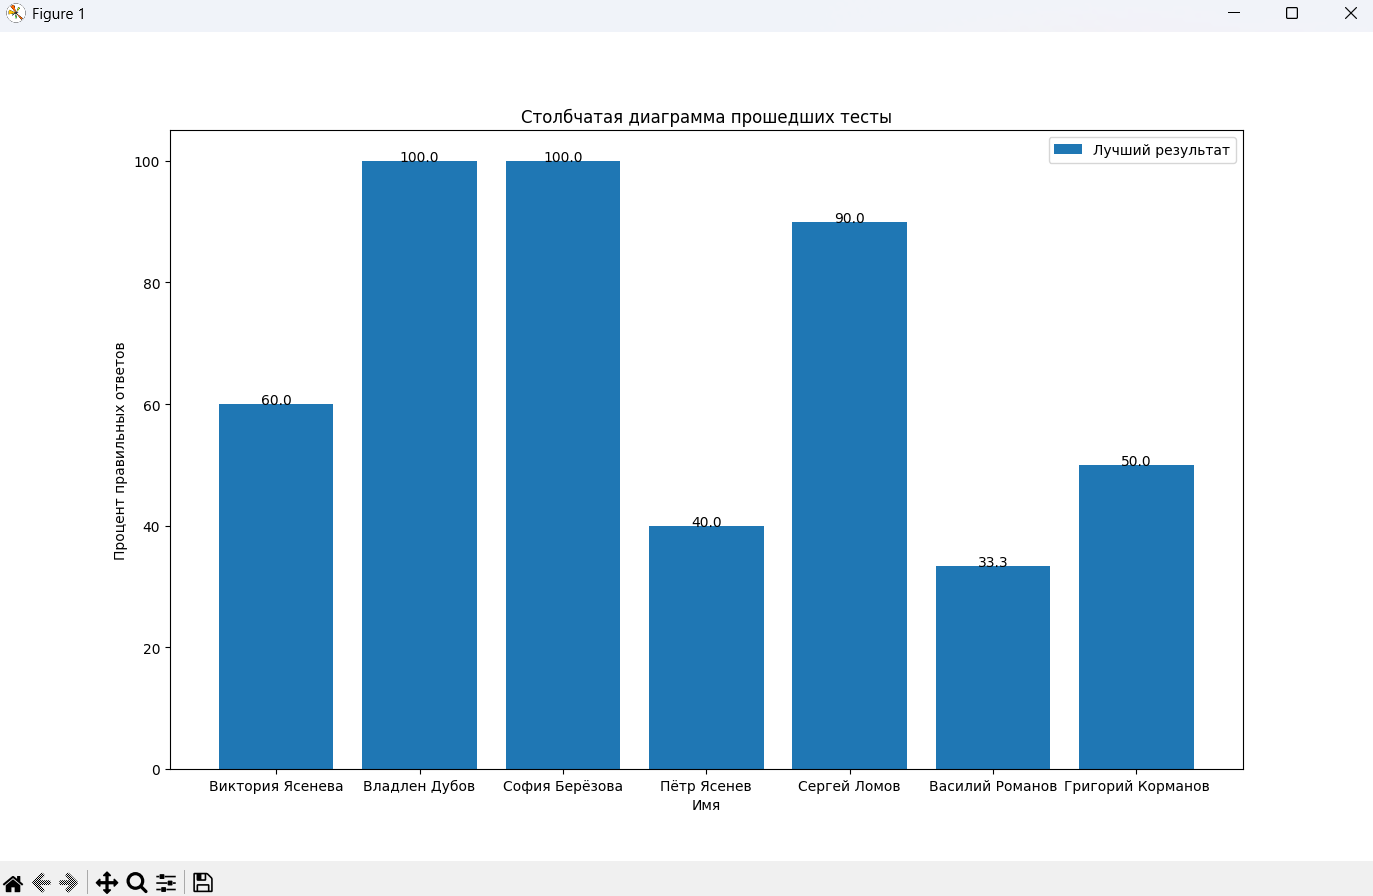
\includegraphics[width=1\linewidth]{результаты_диаграмма.png}
	\caption{Диаграмма результатов}
	\label{results_chart:image}
\end{figure}
\begin{figure}[H]
	\centering
	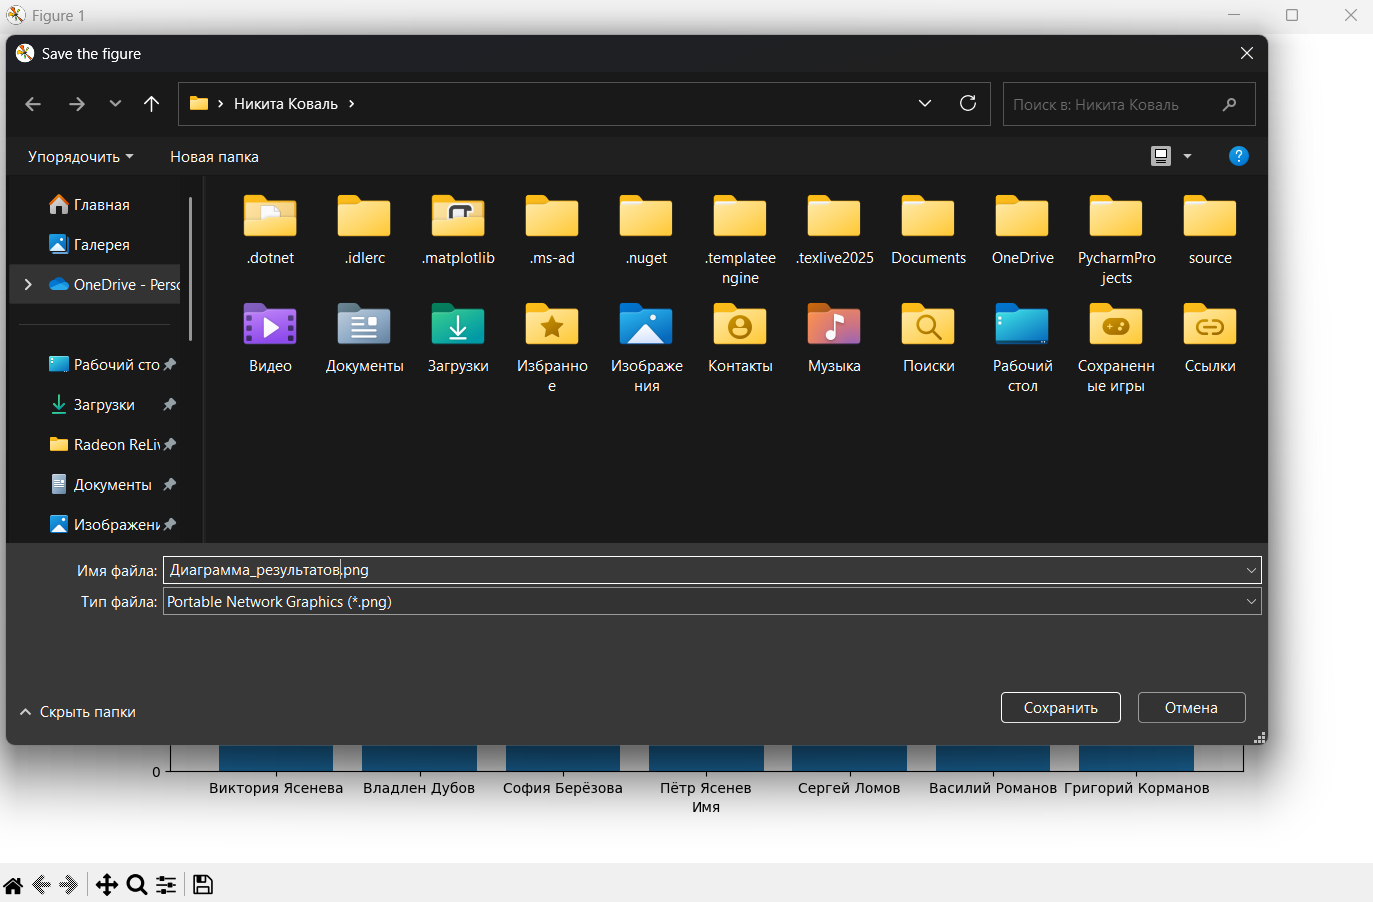
\includegraphics[width=1\linewidth]{сохранение_диаграммы_результатов.png}
	\caption{Диаграмма результатов}
	\label{saving_chart:image}
\end{figure}

\paragraph{Вариант использования <<Удаление вопроса>>}

Заинтересованные лица и их требования: администратор желает удалить вопрос из выбранного теста.
\newline Предусловие: открыто окно "<Меню администратора">.
\newline Постусловие: открыто окно "<Список вопросов">, отображены все вопросы выбранного теста, вопрос удалён.
\newline Основной успешный сценарий:
\begin{enumerate}
	\item Администратор выбирает тест, из которого хочет удалить вопрос (см. рисунок ~\ref{select_test:image}).
	\item Администратор переходит в окно "<Список вопросов">.
	\item Приложение отображает соответствующее окно, где отображены все вопросы выбранного теста (см. рисунок ~\ref{questions_window:image}).
	\item Администратор вводит номер удаляемого вопроса и нажимает кнопку "<Удалить вопрос"> (см. рисунок ~\ref{deleting_complete:image}).
	\item Приложение удаляет вопрос, обновляет список вопросов, сообщает администратору об успешном удалении вопроса и напоминает сохранить изменения (см. рисунок ~\ref{deleting_complete:image}).
	\item Администратор нажимает кнопку "<Сохранить изменения">.
	\item Приложение уведомляет администратора об успешном сохранении изменений (см. рисунок ~\ref{save_notification:image}).
\end{enumerate}

\begin{figure}[H]
	\centering
	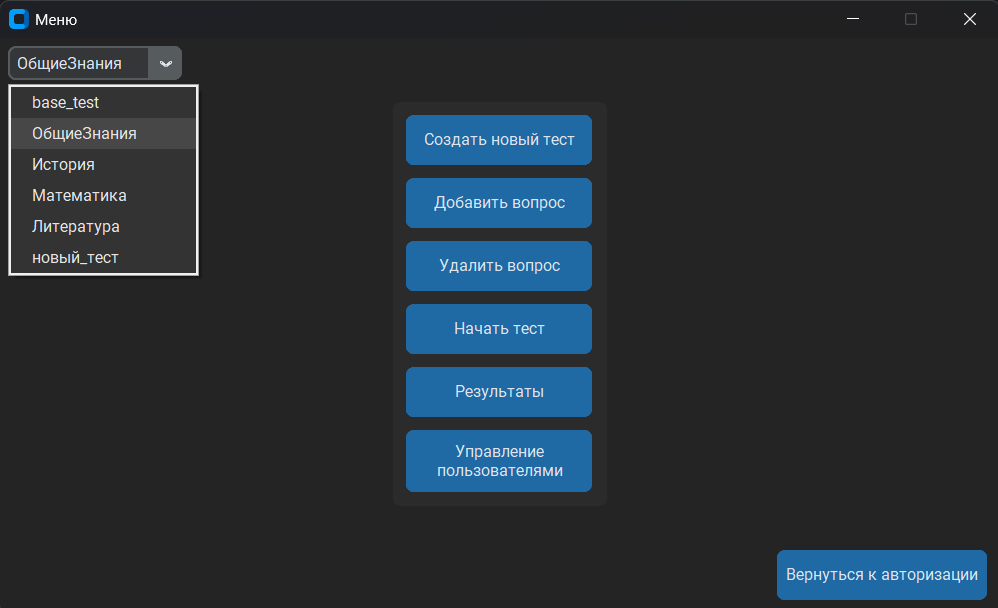
\includegraphics[width=1\linewidth]{выбор_теста.png}
	\caption{Выбор теста в окне "<Меню администратора">}
	\label{select_test:image}
\end{figure}
\begin{figure}[H]
	\centering
	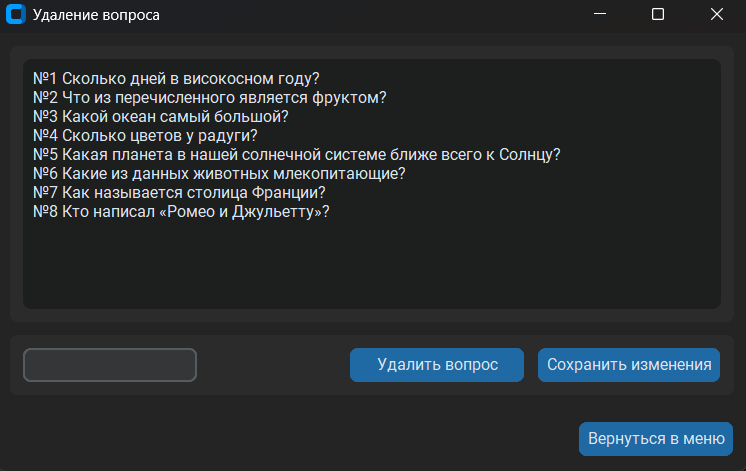
\includegraphics[width=1\linewidth]{вопросы.png}
	\caption{Окно "<Список вопросов">}
	\label{questions_window:image}
\end{figure}
\begin{figure}[H]
	\centering
	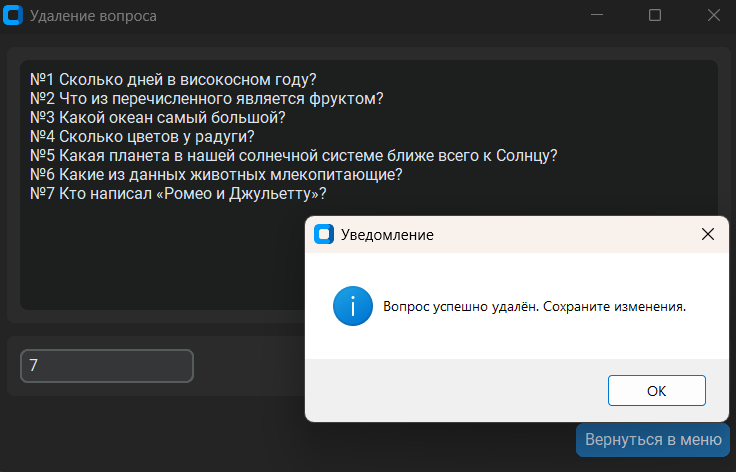
\includegraphics[width=1\linewidth]{сообщение_об_удалении_вопроса.png}
	\caption{Уведомление об удалении вопроса}
	\label{deleting_complete:image}
\end{figure}
\begin{figure}[H]
	\centering
	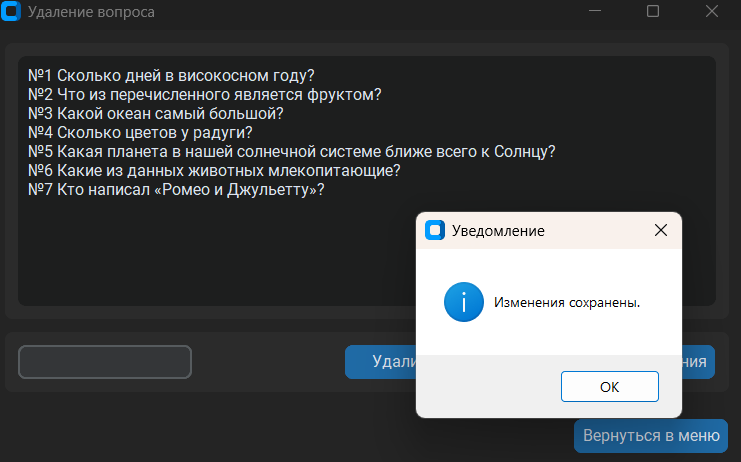
\includegraphics[width=1\linewidth]{сохранение_изменений_уд.png}
	\caption{Уведомление об успешном сохранении изменений}
	\label{save_notification:image}
\end{figure}

\paragraph{Вариант использования <<Создание пользователя администратором>>}

Заинтересованные лица и их требования: администратор желает добавить нового пользователя.
\newline Предусловие: открыто окно "<Меню администратора">.
\newline Постусловие: открыто окно "<Управление пользователями">, отображены все зарегистрированные пользователи, добавлен новый пользователь.
\newline Основной успешный сценарий:
\begin{enumerate}
	\item Администратор переходит в окно "<Управление пользователями">.
	\item Приложение отображает соответствующее окно, где отображены все зарегистрированные пользователи. (см. рисунок ~\ref{users:image}).
	\item Администратор нажимает кнопку "<Добавить пользователя">.
	\item Приложение отображает окно "<Создание пользователя"> (см. рисунок ~\ref{create_user:image}).
	\item Администратор заполняет имя и пароль нового пользователя и нажимает кнопку "<Создать"> (см. рисунок ~\ref{created_user:image}).
	\item Приложение уведомляет администратора об успешном создании нового пользователя (см. рисунок ~\ref{notification_user_created:image}).
\end{enumerate}

\begin{figure}[H]
	\centering
	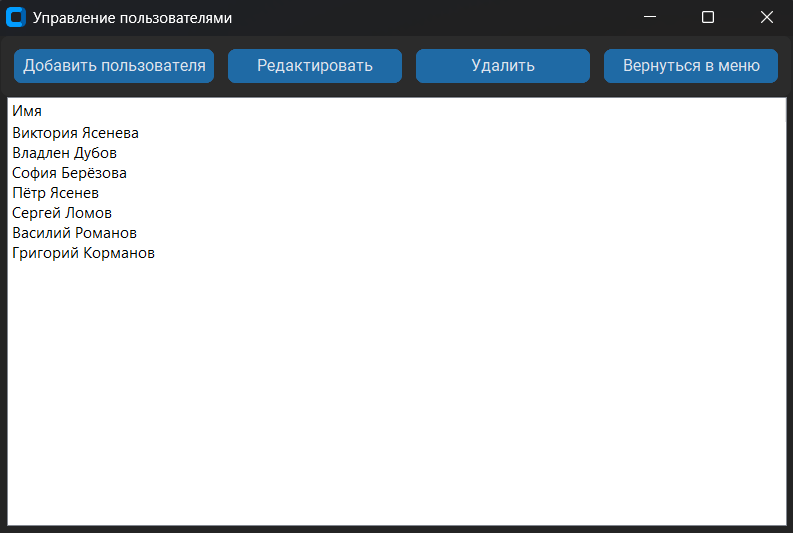
\includegraphics[width=1\linewidth]{управление_пользователями.png}
	\caption{Окне "<Управление пользователями">}
	\label{users:image}
\end{figure}
\begin{figure}[H]
	\centering
	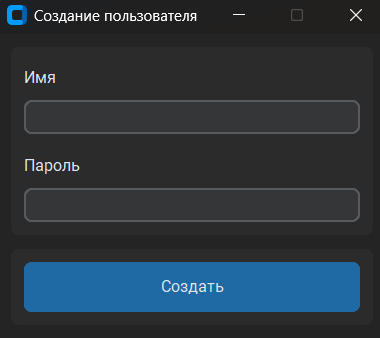
\includegraphics[width=0.6\linewidth]{создание_пользователя.png}
	\caption{Окне "<Создание пользователя">}
	\label{create_user:image}
\end{figure}
\begin{figure}[H]
	\centering
	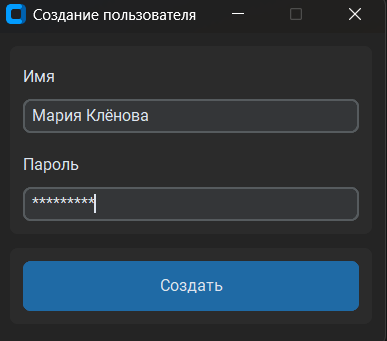
\includegraphics[width=0.6\linewidth]{соз_нов_пол_заполнено.png}
	\caption{Заполнение имени и пароля нового пользователя}
	\label{created_user:image}
\end{figure}
\begin{figure}[H]
	\centering
	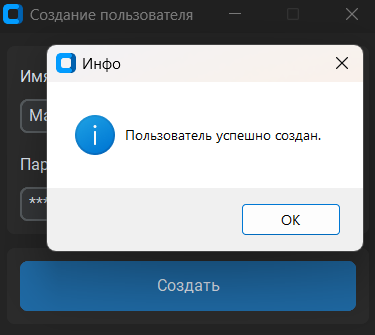
\includegraphics[width=0.6\linewidth]{пользователь_создан_уведомление.png}
	\caption{Уведомление об успешном создании нового пользователя}
	\label{notification_user_created:image}
\end{figure}

\paragraph{Вариант использования <<Удаление пользователя администратором>>}

Заинтересованные лица и их требования: администратор желает удалить пользователя.
\newline Предусловие: открыто окно "<Меню администратора">.
\newline Постусловие: открыто окно "<Управление пользователями">, отображены все зарегистрированные пользователи, пользователь удалён.
\newline Основной успешный сценарий:
\begin{enumerate}
	\item Администратор переходит в окно "<Управление пользователями">.
	\item Приложение отображает соответствующее окно, где отображены все зарегистрированные пользователи.
	\item Администратор выбирает пользователя, которого хочет удалить, и нажимает кнопку "<Удалить"> (см. рисунок ~\ref{deleting_user:image}).
	\item Приложение удаляет пользователя, обновляет список и уведомляет администратора об успешном удалении (см. рисунок ~\ref{user_deleted_notif:image}).
\end{enumerate}

\begin{figure}[H]
	\centering
	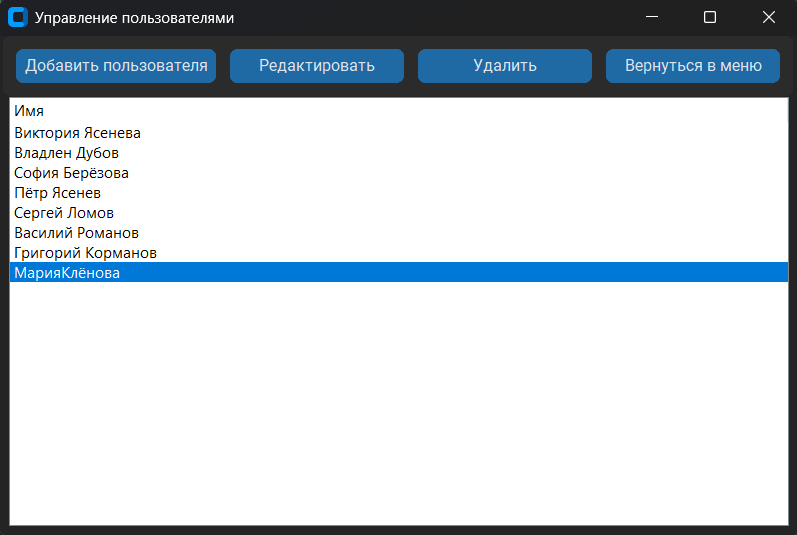
\includegraphics[width=1\linewidth]{удаление_пользователя.png}
	\caption{Удаление выбранного пользователя}
	\label{deleting_user:image}
\end{figure}
\begin{figure}[H]
	\centering
	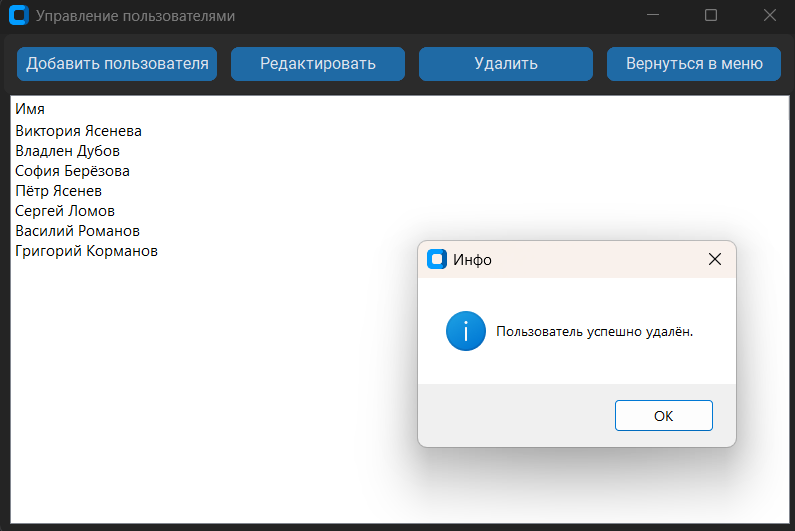
\includegraphics[width=1\linewidth]{пользователь_удалён.png}
	\caption{Уведомление об удалении пользователя}
	\label{user_deleted_notif:image}
\end{figure}

\paragraph{Вариант использования <<Редактирование пользователя администратором>>}

Заинтересованные лица и их требования: администратор желает редактировать пользователя.
\newline Предусловие: открыто окно "<Меню администратора">.
\newline Постусловие: открыто окно "<Управление пользователями">, отображены все зарегистрированные пользователи, изменены имя и пароль пользователя.
\newline Основной успешный сценарий:
\begin{enumerate}
	\item Администратор переходит в окно "<Управление пользователями">.
	\item Приложение отображает соответствующее окно, где отображены все зарегистрированные пользователи.
	\item Администратор выбирает пользователя, которого хочет отредактировать, и нажимает кнопку "<Редактировать"> (см. рисунок ~\ref{edit_user:image}).
	\item Приложение отображает окно с текущими данными пользователя, доступными для редактирования (см. рисунок ~\ref{edit_user_window:image}).
	\item Администратор изменяет имя и пароль пользователя, затем нажимает кнопку "<Сохранить изменения"> (см. рисунок ~\ref{edit_user_1:image}).
	\item Приложение сохраняет изменения, обновляет список пользователей и уведомляет администратора об изменении данных пользователя (см. рисунок ~\ref{edit_user_1:image}).
	\item Результат редактирования данных пользователя (см. рисунок ~\ref{edit_user_2:image})
\end{enumerate}

\begin{figure}[H]
	\centering
	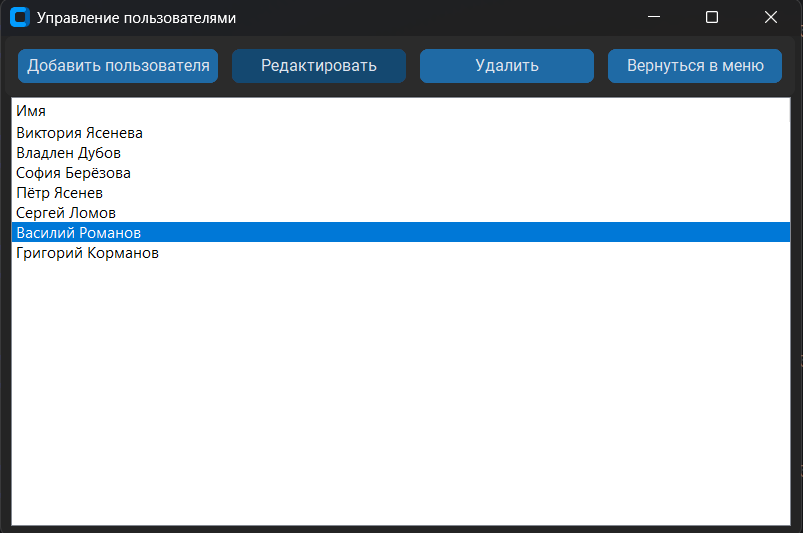
\includegraphics[width=1\linewidth]{ред_пользователя.png}
	\caption{Редактирование выбранного пользователя}
	\label{edit_user:image}
\end{figure}
\begin{figure}[H]
	\centering
	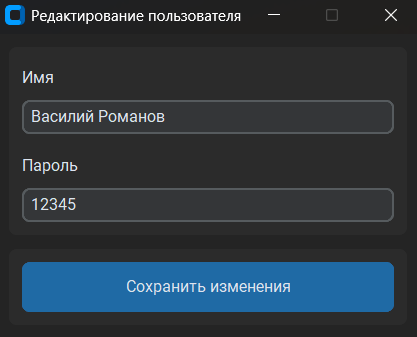
\includegraphics[width=0.6\linewidth]{ред_пол_окно.png}
	\caption{Окно "<Редактирование пользователя">}
	\label{edit_user_window:image}
\end{figure}
\begin{figure}[H]
	\centering
	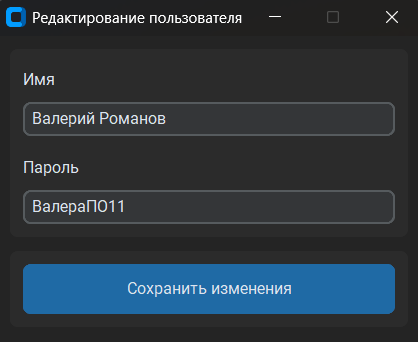
\includegraphics[width=0.6\linewidth]{ред_пол_1.png}
	\caption{Администратор меняет данные пользователя}
	\label{edit_user_1:image}
\end{figure}
\begin{figure}[H]
	\centering
	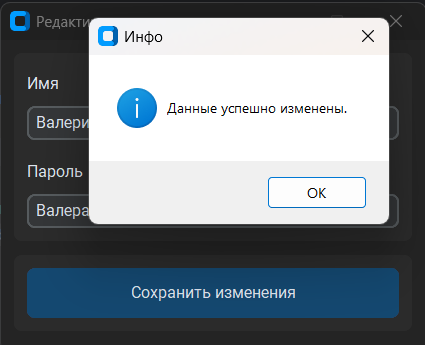
\includegraphics[width=0.6\linewidth]{данные_изменены_ув.png}
	\caption{Уведомление об изменении данных пользователя}
	\label{edit_user_notif:image}
\end{figure}
\begin{figure}[H]
	\centering
	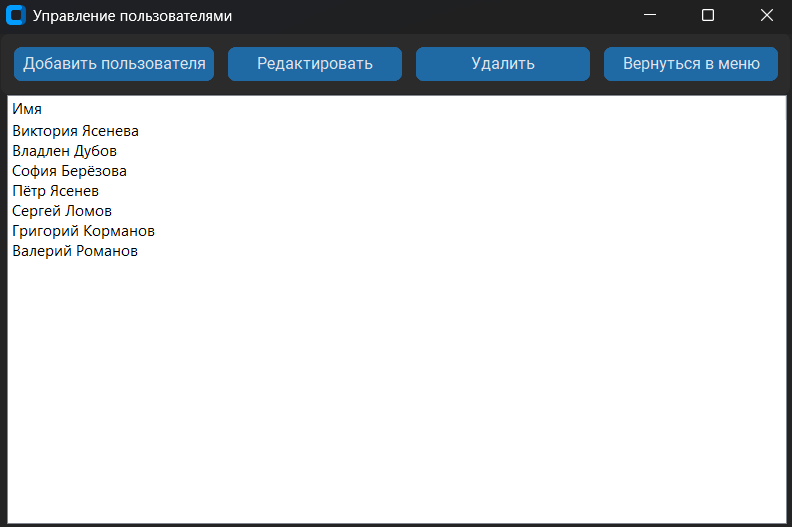
\includegraphics[width=1\linewidth]{изм_данных_пол_1.png}
	\caption{Результат редактирования данных}
	\label{edit_user_2:image}
\end{figure}

\paragraph{Вариант использования <<Создание нового теста и добавление в него вопроса с единственным выбором>>}

Заинтересованные лица и их требования: администратор желает создать новый тест и добавить в него вопрос.
\newline Предусловие: открыто окно "<Меню администратора">.
\newline Постусловие: Создан и сохранён новый тест с добавленным вопросом.
\newline Основной успешный сценарий:
\begin{enumerate}
	\item Администратор переходит в окно "<Создать тест">.
	\item Приложение отображает окно с двумя кнопками: "<Создать новый тест"> и "<Копировать текущий">.
	\item Администратор вводит имя нового теста и нажимает кнопку "<Создать новый тест"> (см. рисунок ~\ref{new_test_window:image}).
	\item Приложение оповещает администратора об успешном создании теста. 
	\item Администратор возвращается в меню, где выбирает созданный тест в выпадающем списке и нажимает кнопку "<Добавить вопрос"> (см. рисунок ~\ref{menu_new_test_window:image}).
	\item Приложение отображает окно "<Выбор типа вопроса"> с тремя кнопками: "<Вопрос с вводом">, "<Вопрос с единственным выбором"> и "<Вопрос с множественным выбором"> (см. рисунок ~\ref{question_selection:image}).
	\item Администратор нажимает кнопку добавить "<Вопрос с единственным выбором">.
	\item Приложение отображает окно для создания соответствующего вопроса.
	\item Администратор заполняет поле ввода для текста вопроса и переходит к созданию списка ответов: вводит ответ на вопрос и при помощи галочки в элементе интерфейса CheckBox указывает правильность ответа. В данном типе вопроса правильный ответ может быть только один. После чего нажимает кнопку "<Добавить ответ"> (см. рисунок ~\ref{radio_question:image}).
	\item Приложение отображает добавленный ответ и отмечает его зелёным цветом, если при создании он был выбран правильным.
	\item После добавления необходимого количества вопросов администратор нажимает кнопку "<Добавить вопрос">.
	\item Приложение добавляет вопрос с введённым текстом и созданным списком ответов в выбранный тест.
	\item Администратор нажимает кнопку "<Сохранить изменения">.
\end{enumerate}

\begin{figure}[H]
	\centering
	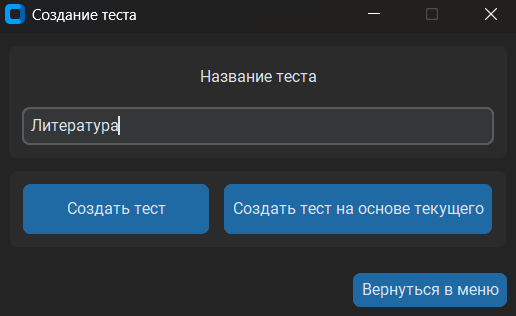
\includegraphics[width=0.7\linewidth]{новый_тест.png}
	\caption{Окно "<Создание теста">}
	\label{new_test_window:image}
\end{figure}
\begin{figure}[H]
	\centering
	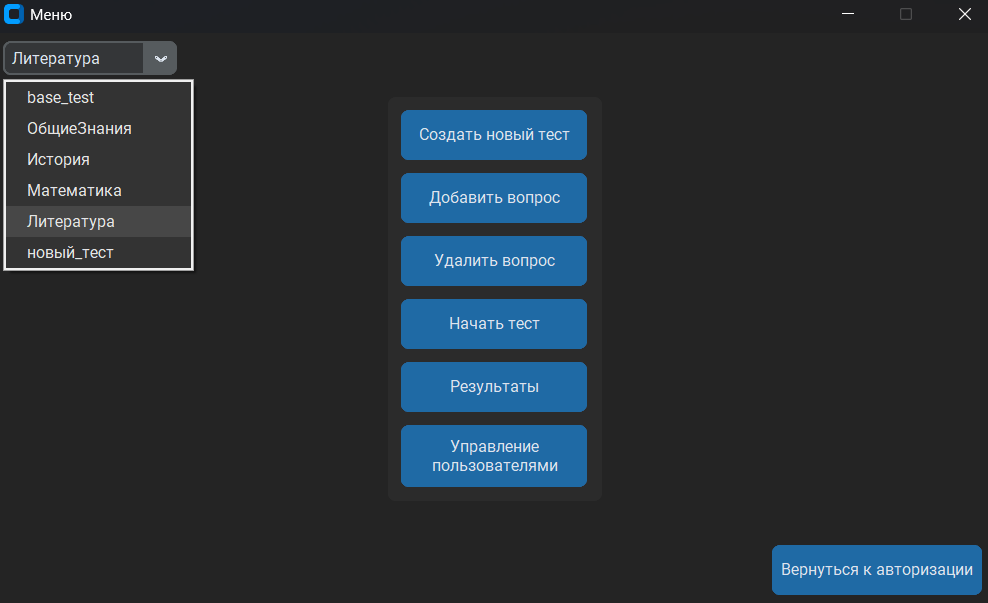
\includegraphics[width=1\linewidth]{меню_выбор_нового_теста.png}
	\caption{Выбор созданного теста в окне "<Меню администратора">}
	\label{menu_new_test_window:image}
\end{figure}
\begin{figure}[H]
	\centering
	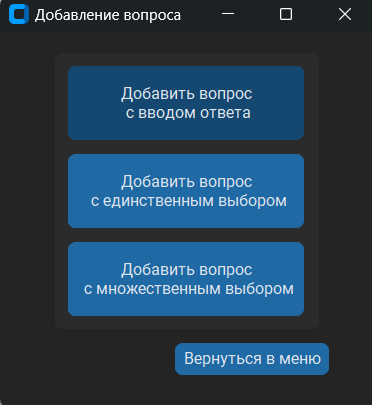
\includegraphics[width=0.6\linewidth]{выбор_типа_вопроса.png}
	\caption{Выбор типа создаваемого вопроса в окне "<Выбор типа вопроса">}
	\label{question_selection:image}
\end{figure}
\begin{figure}[H]
	\centering
	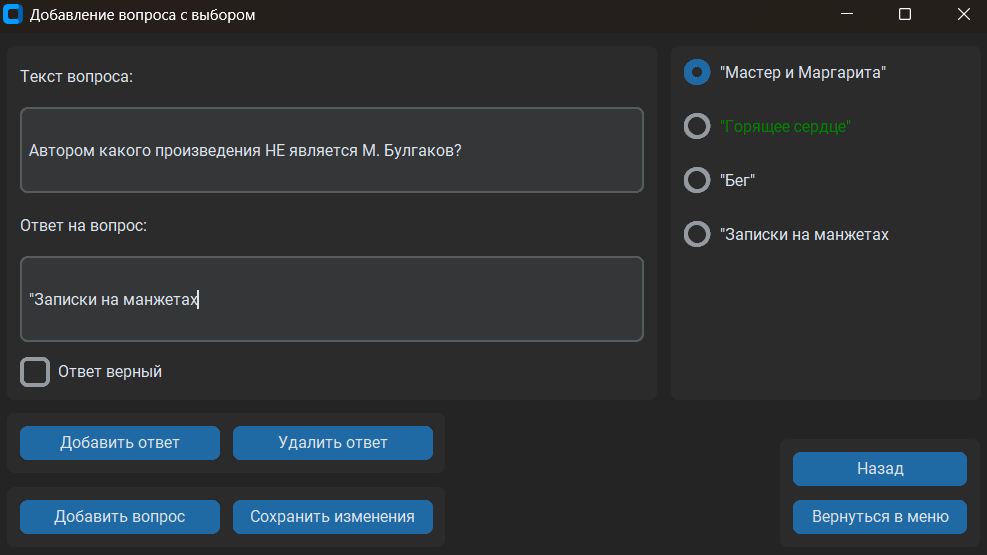
\includegraphics[width=1\linewidth]{добавление_вопроса_с_выбором.png}
	\caption{Окно "<Добавление вопроса с выбором">}
	\label{radio_question:image}
\end{figure}

\paragraph{Вариант использования <<Добавление нового вопроса с вводом ответа>>}

Заинтересованные лица и их требования: администратор желает добавить в тест новый вопрос с вводом ответа.
\newline Предусловие: открыто окно "<Меню администратора">.
\newline Постусловие: В выбранный администратором тест добавлен новый вопрос с вводом ответа.
\newline Основной успешный сценарий:
\begin{enumerate}
	\item Администратор выбирает желаемый тест в выпадающем списке и нажимает кнопку "<Добавить вопрос"> (см. рисунок ~\ref{select_test_1:image}).
	\item Приложение отображает окно "<Выбор типа вопроса"> с тремя кнопками: "<Вопрос с вводом ответа">, "<Вопрос с единственным выбором"> и "<Вопрос с множественным выбором"> (см. рисунок ~\ref{question_selection:image}).
	\item Администратор нажимает кнопку добавить "<Вопрос с вводом ответа">.
	\item Приложение отображает окно для создания соответствующего вопроса (см. рисунок ~\ref{adding_baseQuestion_window:image}).
	\item Администратор заполняет поле ввода для текста вопроса и поле ввода для ответа. После чего нажимает кнопку "<Добавить вопрос"> (см. рисунок ~\ref{adding_baseQuestion_1:image}).
	\item Приложение проверяет, что все поля заполнены, уведомляет администратора об успешном добавлении вопроса и напоминает сохранить изменения (см. рисунок ~\ref{adding_baseQuestion_2:image}).
	\item Администратор нажимает кнопку "<Сохранить изменения">.
	\item Приложение сохраняет изменения и выводит уведомление (см. рисунок ~\ref{adding_baseQuestion_3:image}).
\end{enumerate}

\begin{figure}[H]
	\centering
	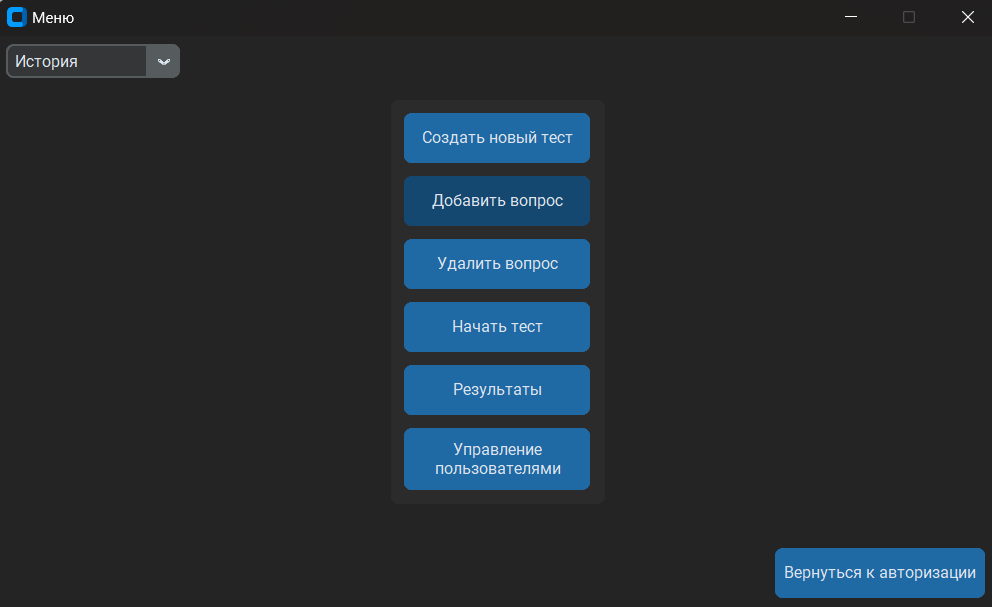
\includegraphics[width=1\linewidth]{выбор_теста_1.png}
	\caption{Выбор теста "<История"> и нажатие кнопки "<Добавить вопрос">}
	\label{select_test_1:image}
\end{figure}
\begin{figure}[H]
	\centering
	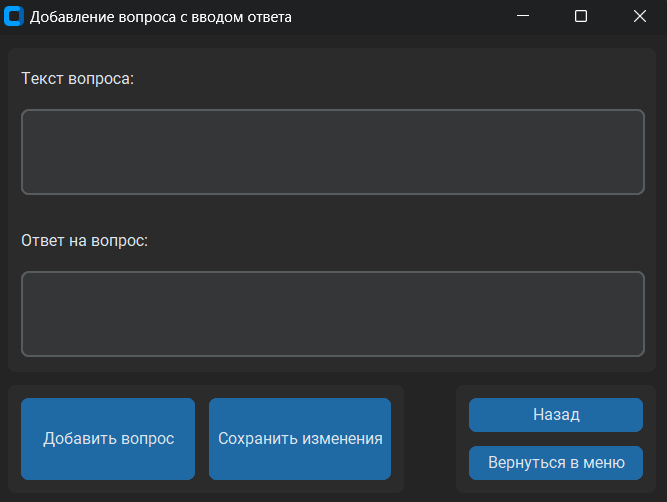
\includegraphics[width=0.6\linewidth]{доб_вопроса_с_вводом_окно.png}
	\caption{Окно "<Добавление вопроса с вводом ответа">}
	\label{adding_baseQuestion_window:image}
\end{figure}
\begin{figure}[H]
	\centering
	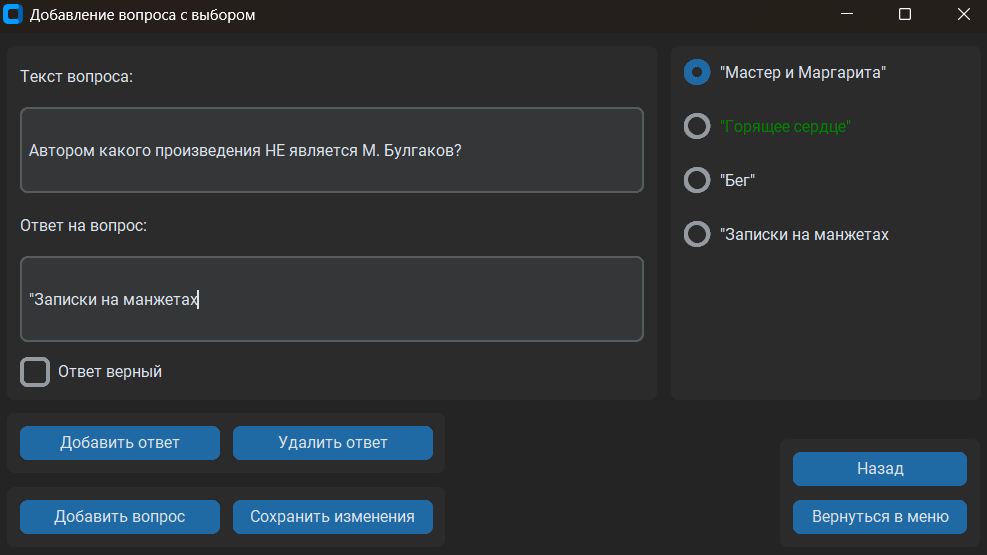
\includegraphics[width=1\linewidth]{добавление_вопроса_с_вводом_1.png}
	\caption{Ввод вопроса и ответа на него}
	\label{adding_baseQuestion_1:image}
\end{figure}
\begin{figure}[ht]
	\centering
	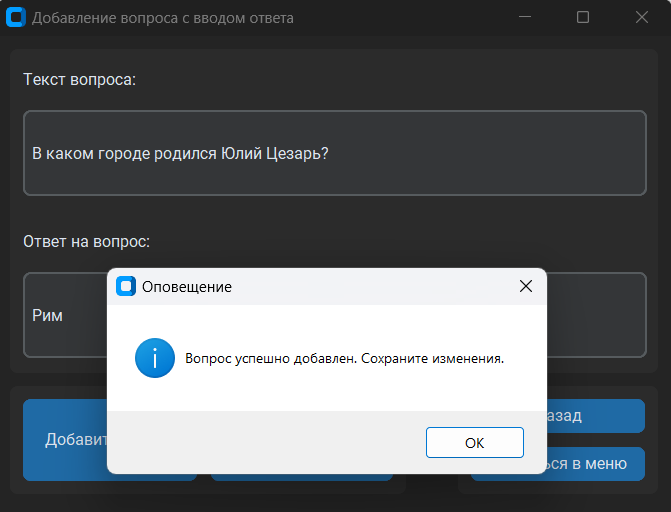
\includegraphics[width=1\linewidth]{доб_воп_ув_1.png}
	\caption{Уведомление об успешном добавлении вопроса}
	\label{adding_baseQuestion_2:image}
\end{figure}
\begin{figure}[H]
	\centering
	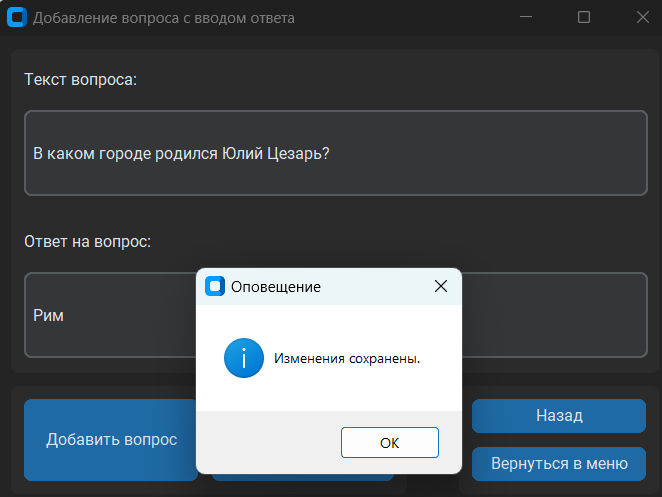
\includegraphics[width=1\linewidth]{уведомление_1.png}
	\caption{Уведомление о сохранении изменений}
	\label{adding_baseQuestion_3:image}
\end{figure}

\paragraph{Вариант использования <<Добавление нового вопроса с множественным выбором ответа>>}

Заинтересованные лица и их требования: администратор желает добавить в тест новый вопрос с множественным выбором ответа.
\newline Предусловие: открыто окно "<Меню администратора">.
\newline Постусловие: В выбранный администратором тест добавлен новый вопрос с множественным выбором ответа.
\newline Основной успешный сценарий:
\begin{enumerate}
	\item Администратор выбирает желаемый тест в выпадающем списке и нажимает кнопку "<Добавить вопрос">.
	\item Приложение отображает окно "<Выбор типа вопроса"> с тремя кнопками: "<Вопрос с вводом ответа">, "<Вопрос с единственным выбором"> и "<Вопрос с множественным выбором"> (см. рисунок ~\ref{question_selection:image}).
	\item Администратор нажимает кнопку добавить "<Вопрос с множественным выбором">.
	\item Приложение отображает окно для создания соответствующего вопроса (см. рисунок ~\ref{question_2:image}).
	\item Администратор заполняет поле ввода для текста вопроса и переходит к созданию списка ответов: вводит ответ на вопрос и при помощи галочки в элементе интерфейса CheckBox указывает правильность ответа. В данном типе вопроса правильных ответов может быть несколько. После чего нажимает кнопку "<Добавить ответ">.
	\item Приложение отображает добавленный ответ и отмечает его зелёным цветом, если при создании он был выбран правильным (см. рисунок ~\ref{question_input:image}).
	\item После добавления необходимого количества вопросов администратор нажимает кнопку "<Добавить вопрос">.
	\item Приложение проверяет, что все поля заполнены, уведомляет администратора об успешном добавлении вопроса и напоминает сохранить изменения (см. рисунок ~\ref{question_3t:image}).
	\item Администратор нажимает кнопку "<Сохранить изменения">.
	\item Приложение сохраняет изменения и выводит уведомление (см. рисунок ~\ref{question_4t:image}).
\end{enumerate}

\begin{figure}[H]
	\centering
	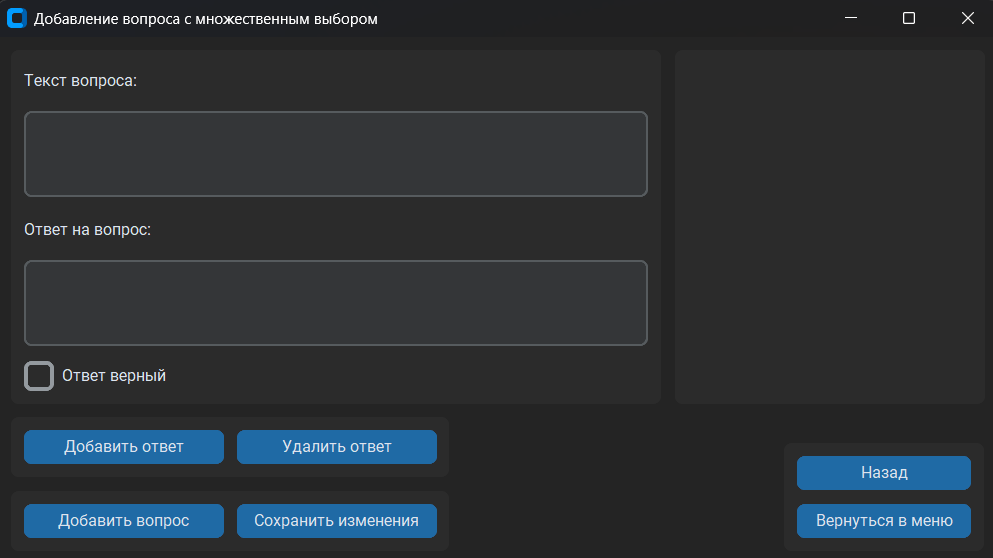
\includegraphics[width=1\linewidth]{вопрос_с_мн_выб.png}
	\caption{Окно "<Добавление вопроса с множественным выбором">}
	\label{question_2:image}
\end{figure}
\begin{figure}[H]
	\centering
	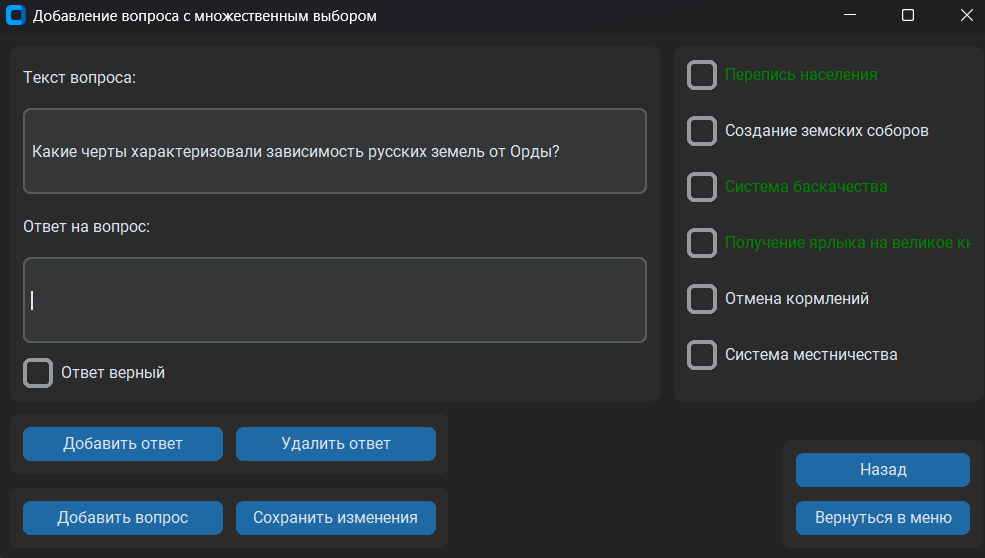
\includegraphics[width=1\linewidth]{ввод_вопроса_с_мн_выб.png}
	\caption{Ввод вопроса с множественным выбором}
	\label{question_input:image}
\end{figure}
\begin{figure}[H]
	\centering
	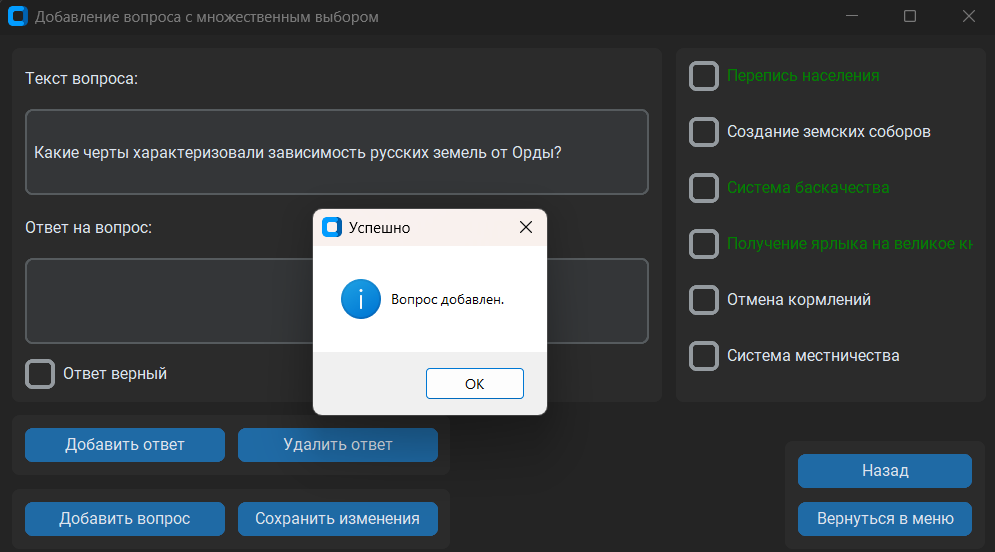
\includegraphics[width=1\linewidth]{доб_вопроса_с_мн_выбором.png}
	\caption{Уведомление о добавлении вопроса}
	\label{question_3t:image}
\end{figure}
\begin{figure}[H]
	\centering
	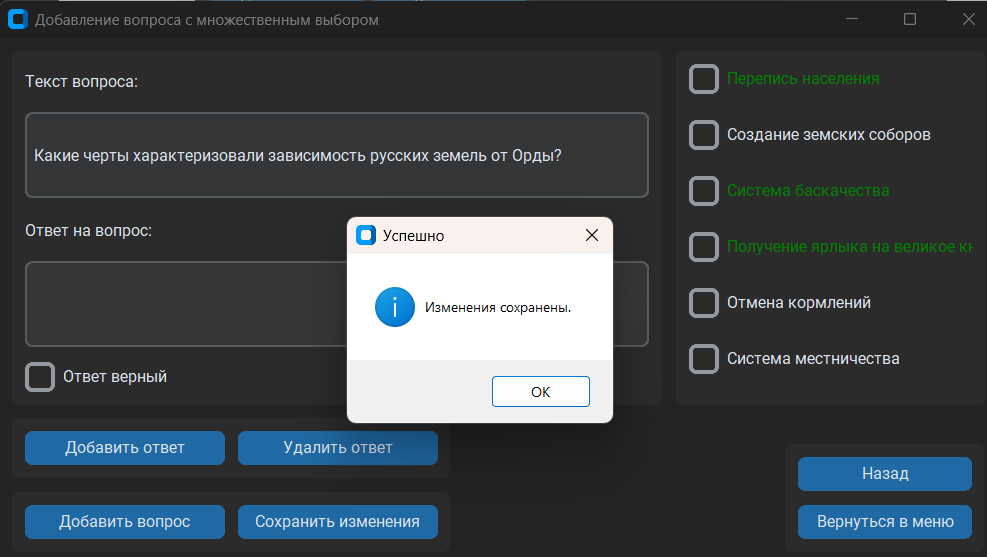
\includegraphics[width=1\linewidth]{доб_воп_3.png}
	\caption{Уведомление о сохранении изменений}
	\label{question_4t:image}
\end{figure}

\subsection{Требования пользователя к интерфейсу приложения}

Приложение должно иметь следующие основные экраны:
\begin{enumerate}
	\item Окно "<Авторизация"> - экран при открытии приложения, где пользователь может ввести имя и пароль для входа в свой аккаунт. Имеет переход в окна: "<Меню пользователя">, "<Регистрация">,  и "<Авторизоваться как администратор">.
	\item Окно "<Регистрация"> - экран приложения, на котором пользователь может зарегистрироваться. Имеет переход в окно "<Авторизация">.
	\item Окно "<Авторизоваться как администратор"> - экран приложения, на котором требуется ввести пароль администратора. После успешного ввода пароля позволяет перейти в специальное меню администратора с расширенными возможностями. Имеет переход в окна: "<Меню администратора">, "<Изменить пароль администратора"> и "<Вернуться к авторизации пользователя">.
	\item Окно "<Изменить пароль администратора"> - экран приложения, на котором пользователь может изменить пароль администратора, требуется ввести старый пароль и два раза новый. Имеет переход к окну "<Авторизоваться как администратор">.
	\item Окно "<Меню пользователя"> - экран приложения, на котором пользователь может выбрать тест и перейти к его прохождению, просмотреть результаты своих завершённых тестов. Имеет переходы в окна: "<Тест">, "<Результаты">.
	\item Окно "<Тест"> - экран приложения, на котором динамически отображаются вопросы теста и требуется ввести или выбрать соответствующий ответ.
	\item Окно "<Результаты"> - экран приложения, на котором в зависимости от прав доступа отображаются результаты пройденных тестов. Для пользователя отображаются только собственные результаты, для администратора - результаты всех пользователей с возможностью создания и выгрузки диаграммы, отображающей лучшие попытки прохождения тестов.
	\item Окно "<Меню администратора"> - экран приложения, на котором доступны все возможности системы тестирования знаний: создание и редактирование тестов, управление пользователями, просмотр и прохождение тестов, результаты тестов всех пользователей. Имеет переходы в окна: "<Создать тест">, "<Добавить вопрос">, "<Список вопросов">, "<Тест">, "<Управление пользователями">, "<Результаты">.
	\item Окно "<Создать тест"> - экран приложения, на котором можно создать новый тест с пустым списком вопросов или копировать список вопросов из выбранного теста. 
	\item Окно "<Добавление вопрос"> - экран приложения, на котором можно добавить три типа вопроса: с вводом ответа, с единственным выбором ответа, с множественным выбором.
	\item Окно "<Удаление вопроса"> - экран приложения, на котором отображен список всех вопросов теста с возможностью удаления любого вопроса из списка.
	\item Окно "<Управление пользователями"> - экран приложения, на котором отображены все зарегистрированные пользователи. Позволяет администратору добавлять, удалять и редактировать пользователей.
\end{enumerate}

\subsection{Требования к оформлению документации}

Разработка программной документации и программного изделия должна производиться согласно ГОСТ 19.102-77 и ГОСТ 34.601-90. Единая система программной документации.
